\section{Example joint posteriors}
\label{app:corner_posteriors}

Figures~\ref{fig:corner_ev_lac}--\ref{fig:corner_gj_1289} show the full joint
posterior distributions of the magnetic spectral fit for three representative
stars, spanning the range of retrieved field strengths in our sample: EV~Lac
(Gl~873), with the strongest field, DS~Leo (Gl~410), among the weakest, and the
intermediate GJ~1289. Each triangle places the magnetic filling-factor simplex
to the left of the five atmospheric parameters, so that the correlations between
the field components and the atmospheric structure can be read off directly. The
width of the simplex --- the number of field bins $a_0,\dots,a_{B_{\rm max}}$ ---
is set per star by the BIC-optimal region-filtered model
(Sect.~\ref{sec:methods_filter}), which is why it differs from figure to figure.

\begin{figure*}[p]
    \centering
    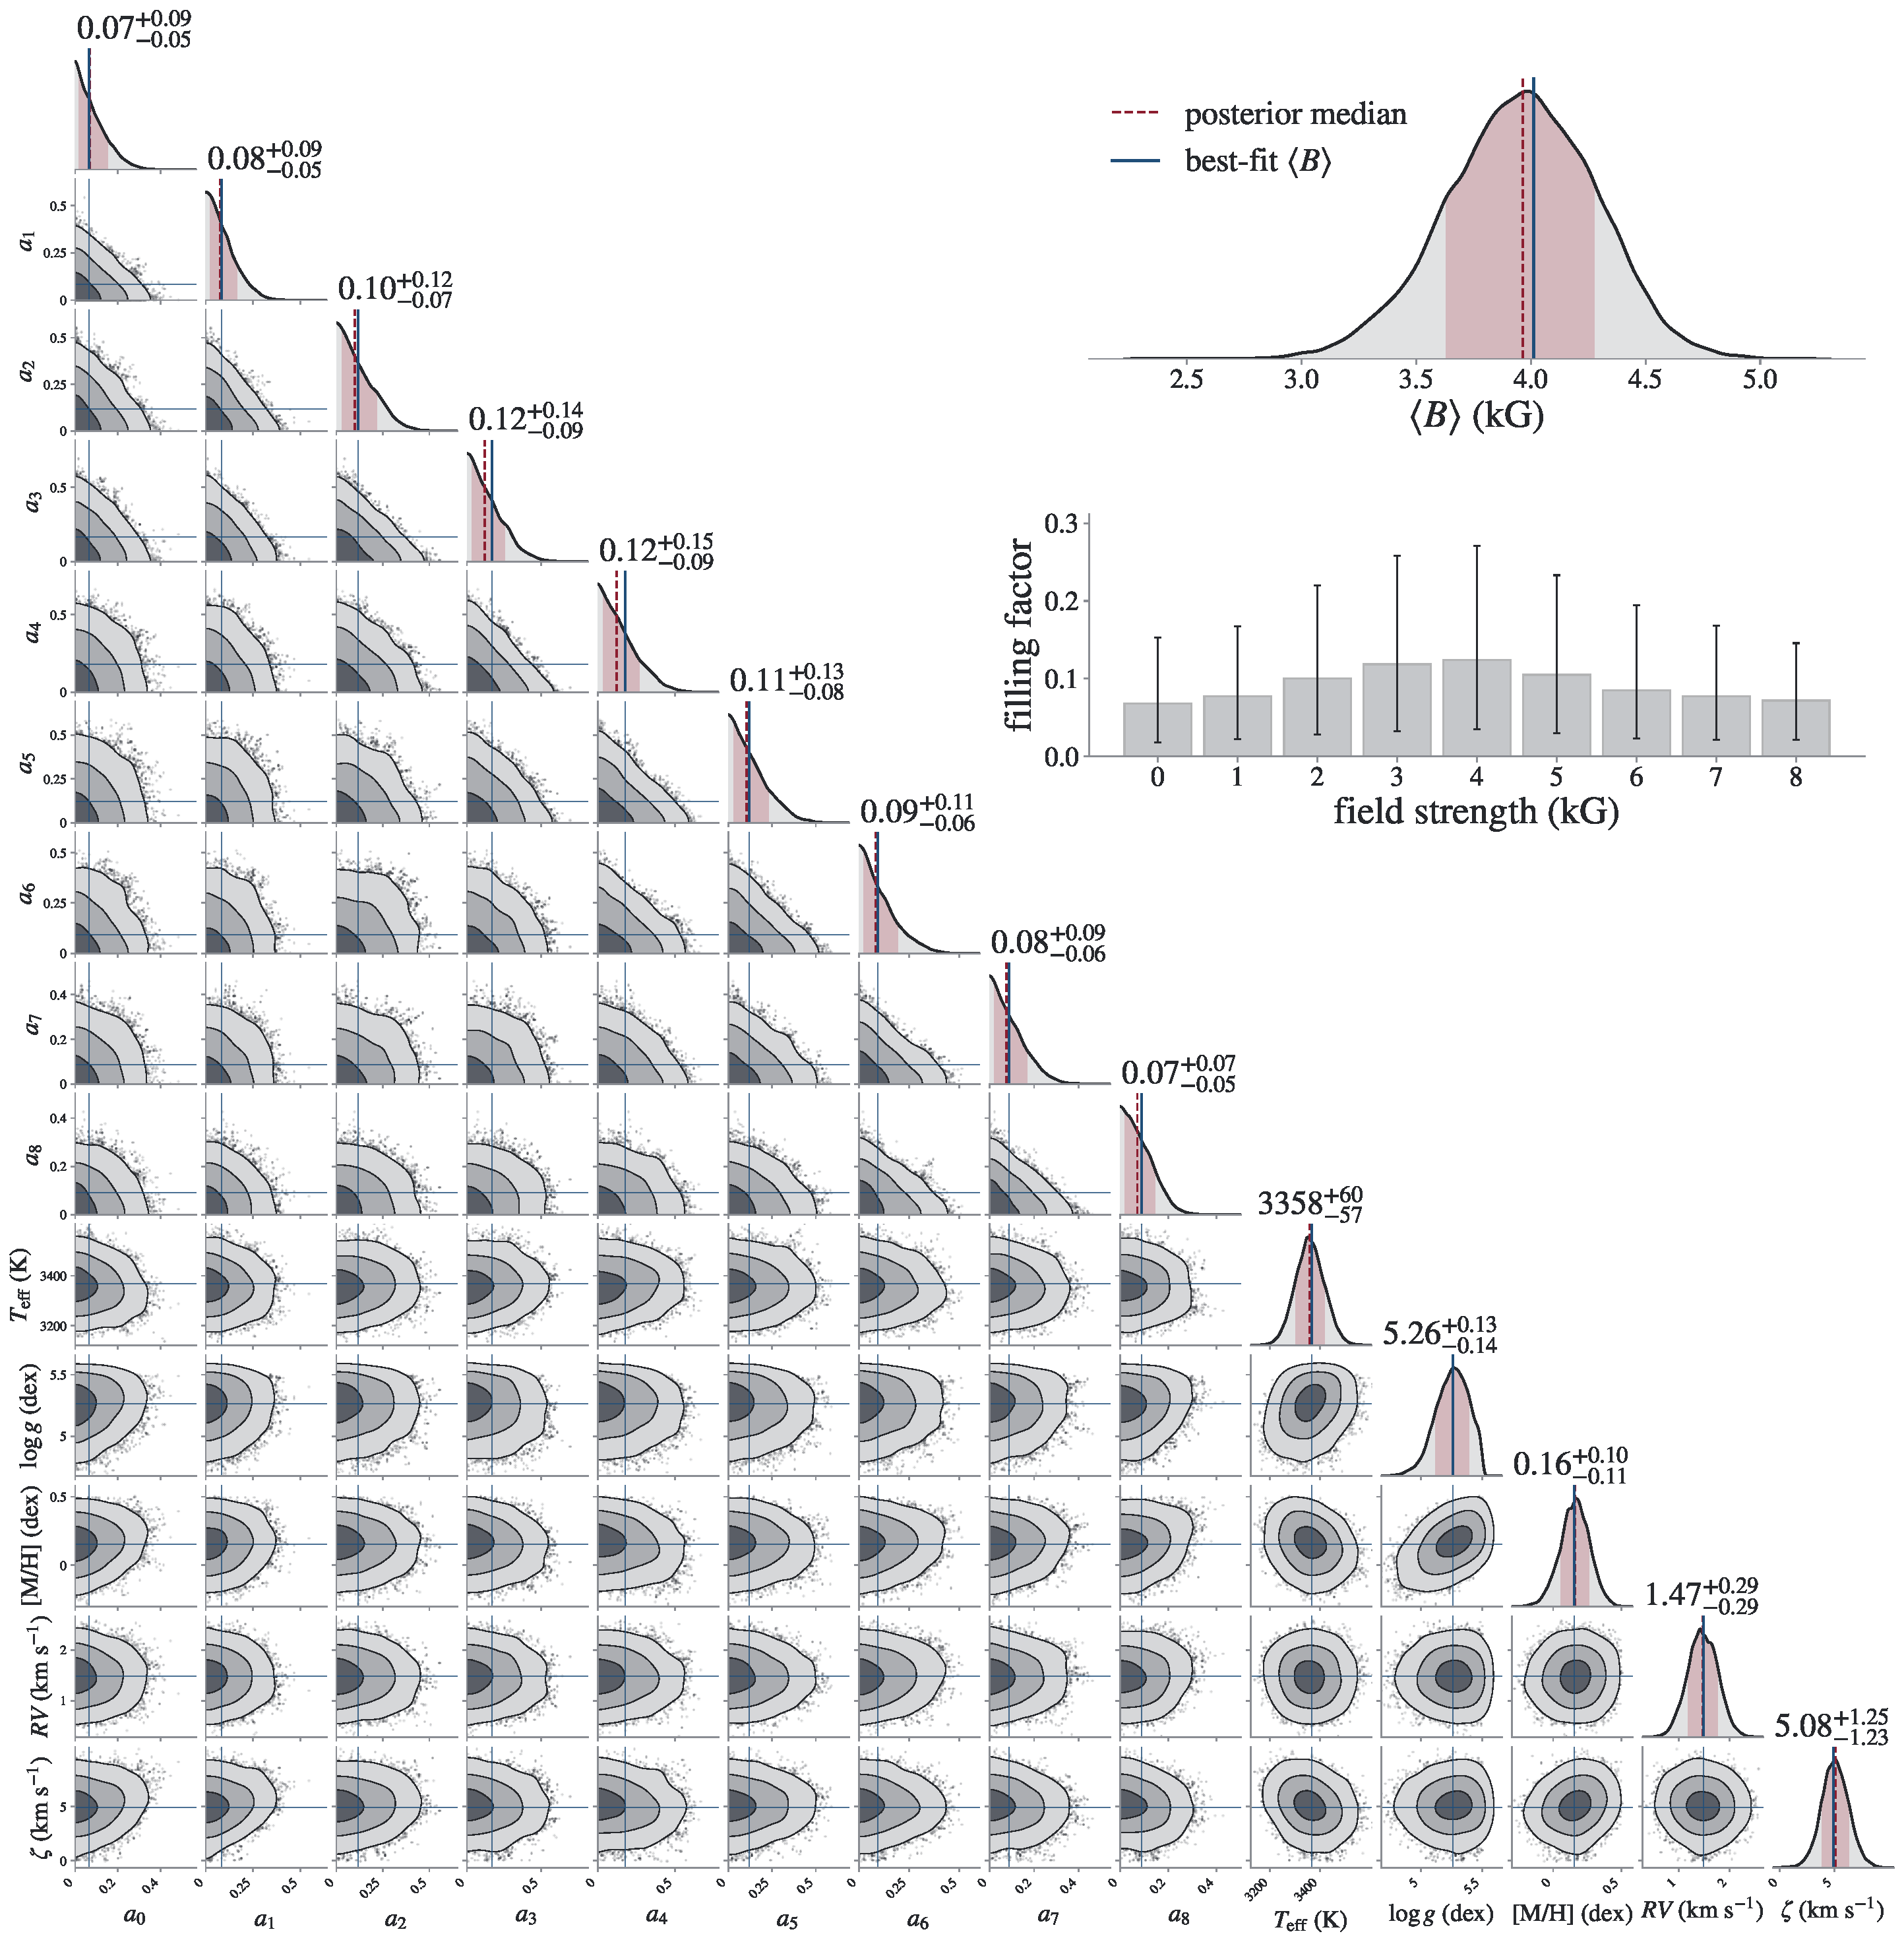
\includegraphics[width=\textwidth]{figures/corner_posterior_ev_lac.pdf}
    \caption{Joint posterior distribution of the magnetic spectral fit to EV~Lac
    (Gl~873) from the Narval template. The triangle shows the magnetic
    filling-factor simplex --- $a_0$ (the $B=0$\,kG closure) through $a_8$, one
    per field bin retained by the BIC-optimal region-filtered model --- followed
    by the five atmospheric parameters ($T_{\rm eff}$, $\log g$, [M/H], $RV$,
    $\zeta$). Diagonal panels give the 1D marginals with the $68\%$ credible
    interval shaded; the dashed crimson line marks the posterior median (quoted
    with $\pm68\%$ above each panel) and the solid steel line the reported
    best-fit value (mean of the highest-likelihood $5\%$ of samples). Off-diagonal
    panels show the 2D joint densities with $1$/$2$/$3\sigma$ contours. The
    upper-right insets show the posterior of the mean field
    $\langle B\rangle = \sum_i a_i B_i$, peaking at
    $\langle B\rangle = 4.0$\,kG, and the marginal filling factor of each field
    bin. The broad, overlapping magnetic marginals reflect the strong
    anti-correlations between adjacent filling factors imposed by the simplex
    closure.}
    \label{fig:corner_ev_lac}
\end{figure*}

\begin{figure*}[p]
    \centering
    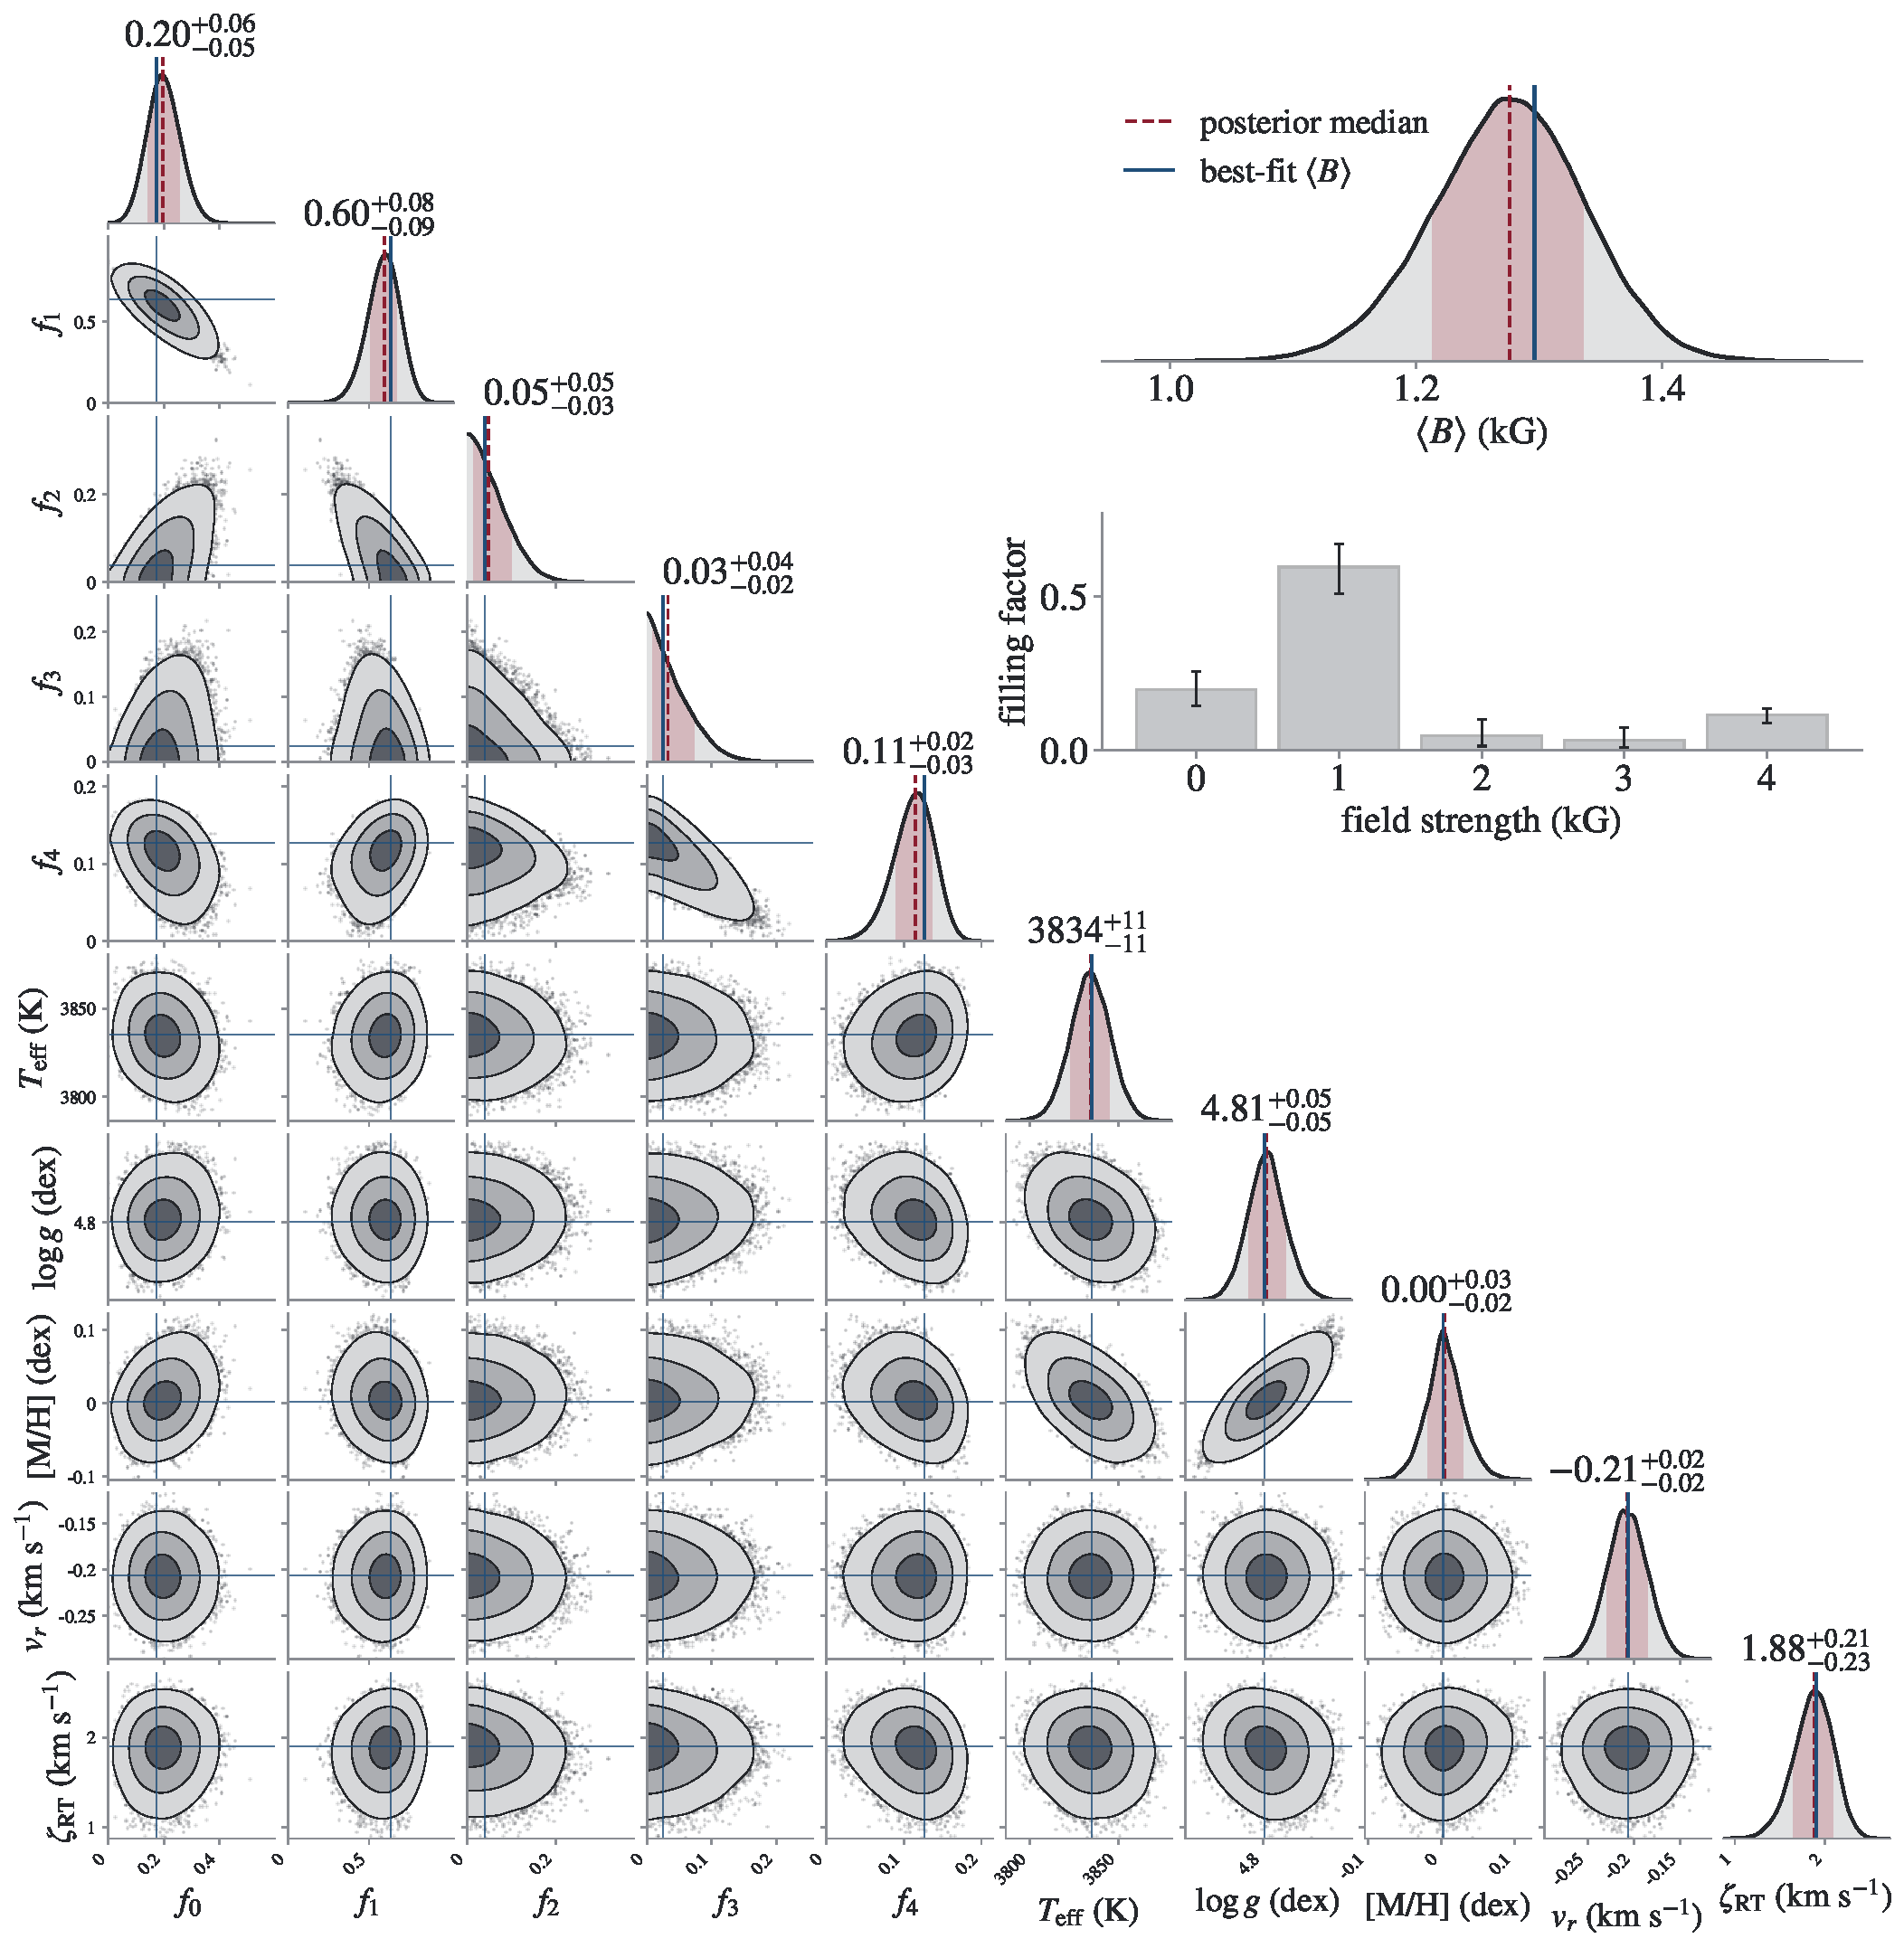
\includegraphics[width=\textwidth]{figures/corner_posterior_ds_leo.pdf}
    \caption{Joint posterior distribution of the magnetic spectral fit to DS~Leo
    (Gl~410) from the Narval template, in the same format as
    Fig.~\ref{fig:corner_ev_lac}. Here the BIC-optimal region-filtered model
    retains a much narrower simplex, $a_0$ (the $B=0$\,kG closure) through $a_4$,
    consistent with this being one of the weakest-field stars in the sample: the
    mean-field posterior in the upper-right inset peaks at
    $\langle B\rangle = 1.3$\,kG, with the bulk of the filling factor sitting in
    the $a_0$ and $a_1$ bins. Panel layout, line styles, shading and contour
    levels are as in Fig.~\ref{fig:corner_ev_lac}.}
    \label{fig:corner_ds_leo}
\end{figure*}

\begin{figure*}[p]
    \centering
    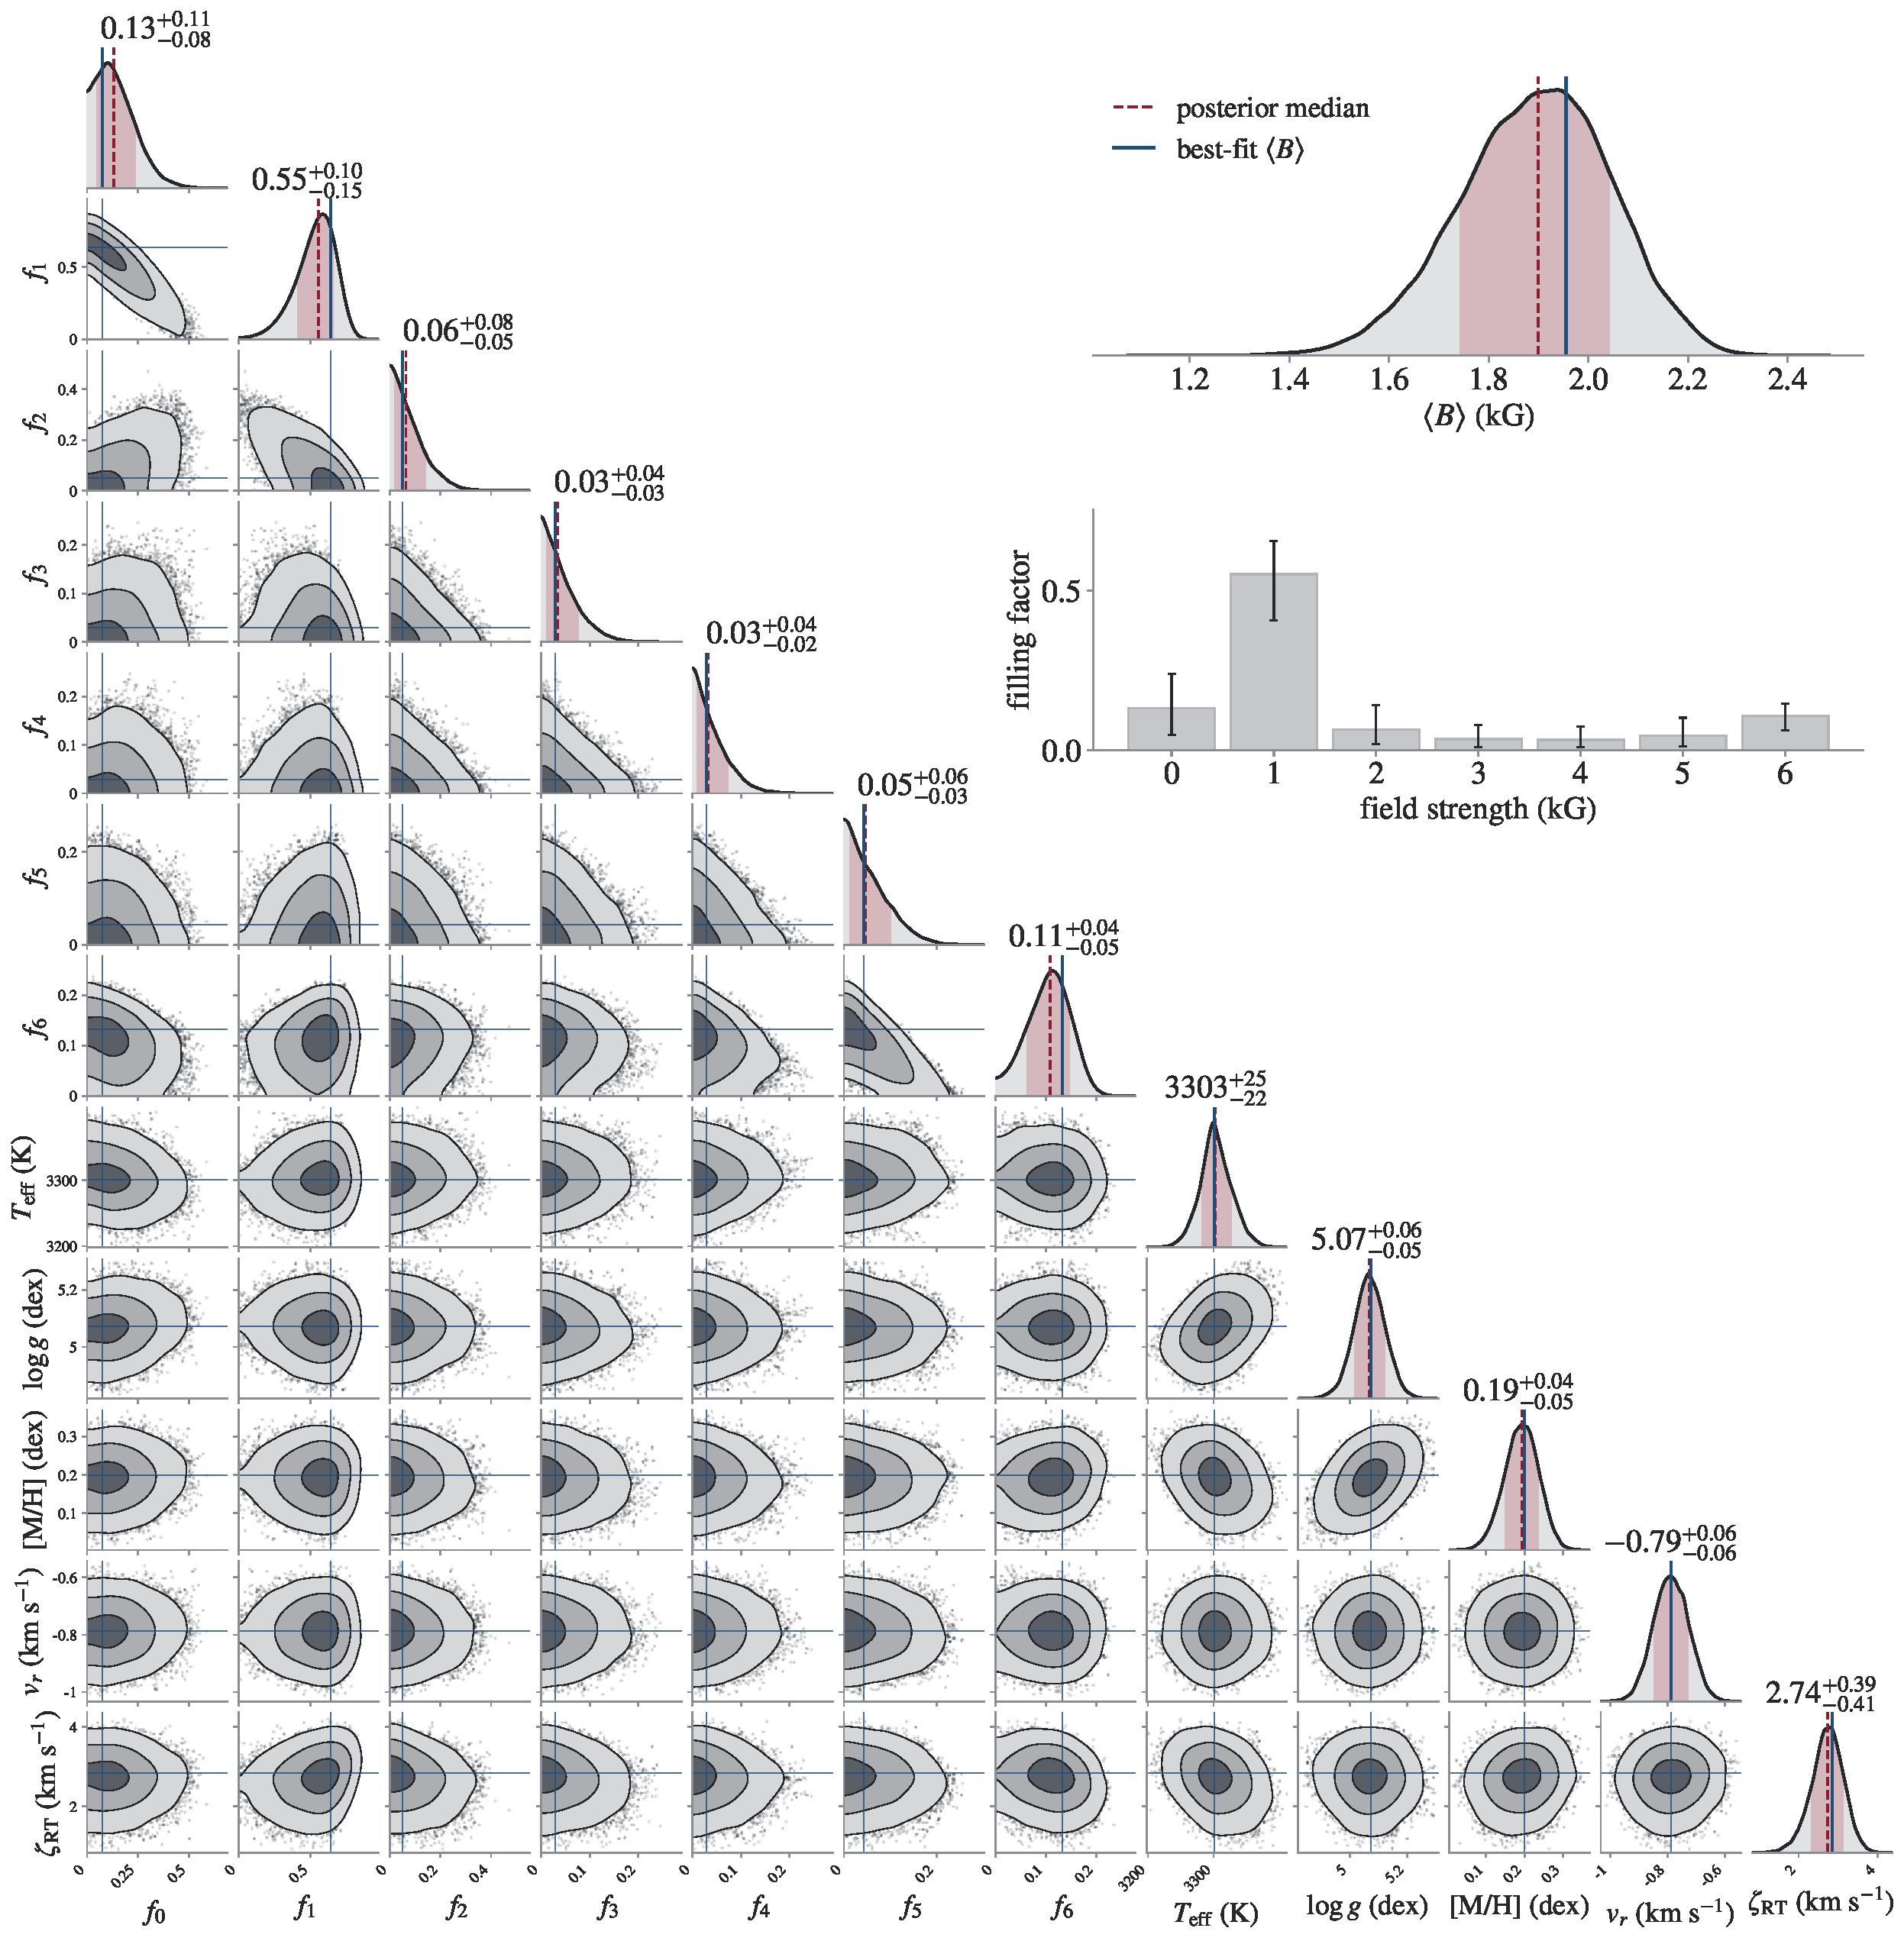
\includegraphics[width=\textwidth]{figures/corner_posterior_gj_1289.pdf}
    \caption{Joint posterior distribution of the magnetic spectral fit to
    GJ~1289 from the Narval template, again following
    Fig.~\ref{fig:corner_ev_lac}. The BIC-optimal region-filtered model keeps an
    intermediate simplex, $a_0$ (the $B=0$\,kG closure) through $a_6$; the
    mean-field posterior in the upper-right inset peaks at
    $\langle B\rangle = 2.0$\,kG. As in the other examples the adjacent magnetic
    marginals are broad and strongly anti-correlated through the simplex closure,
    whereas the atmospheric parameters are comparatively well constrained.}
    \label{fig:corner_gj_1289}
\end{figure*}

\FloatBarrier
